% -*- compile-command: "pdflatex --enable-write18 XXX.tex" -*-
\documentclass{tufte-handout}

\usepackage{algo-activity}

\title{Algorithms: Binomial Heaps}
\date{}

\begin{document}

\maketitle



\begin{objective}
  Students will learn about binomial heaps and analyze their amortized running time.
\end{objective}

\begin{questions}

\item A binomial tree of order 0 is a single node. A binomial tree of order $n$ consists of a root node with $n$ subtrees. The leftmost subtree is of order $n-1$, the next subtree is of order $n-2$, and so forth, with the rightmost subtree of order 0.

Model \ref{binomial-trees} depicts a series of \emph{binomial trees} in increasing order. The leftmost tree is order 0, the next one is order 1, the third one is order 2, the fourth one is order 3, and the final tree is order 4.

\begin{model*}{Binomial Trees}{binomial-trees}
  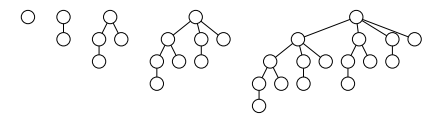
\includegraphics[]{binomial_trees.PNG}
  \label{binomial-trees}
\end{model*}

Prove by induction that a binomial tree of order $n$ has $2^n$ nodes.

\item How can we make a binomial tree of order $n$ from two binomial trees of order $n - 1$? \label{binomial-merge}

\item Give an asymptotic upper bound on the time necessary for the algorithm you wrote for Question \ref{binomial-merge}.

\item A \emph{binomial heap} is a list of binomial trees such that:
\begin{itemize}
    \item Each binomial tree satisfies the heap property, i.e., each node's value is less than or equal to the values of all its children.
    \item There is at most one binomial tree of any given order.
\end{itemize}

\begin{model*}{Binomial Heap}{binomial-heap}
  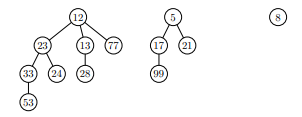
\includegraphics[]{binomial_heap.PNG}
  \label{binomial-heap}
\end{model*}

How many total nodes does the binomial heap in Model \ref{binomial-heap} contain?

\item What is the order of each binomial tree in Model \ref{binomial-heap}?

\item The table in Model \ref{heaptrees} lists a total number of nodes and the number of trees of each order. Fill in the table.

\begin{model*}{Trees in binomial heap of size $n$}{heaptrees}
  \centering
  % \tabcolsep=0.1cm
  \begin{tabular}{c|cccccccccccccccc}
    $n$ & $0$ & $1$ & $2$ & $3$ & $4$ & $5$ & $6$ & $7$ & $8$ & $9$ & $10$
    & $11$ & $12$ & $13$ & $14$ & $15$  \\[8pt]
    Order 0 trees & $0$ & $1$ & $0$ & & & & & & & & & & & & & \\[8pt]
    Order 1 trees & $0$ & $0$ & $1$ & & & & & & & & & & & & & \\[8pt]
    Order 2 trees & $0$ & $0$ & $0$ & & & & & & & & & & & & & \\[8pt]
    Order 3 trees & $0$ & $0$ & $0$ & & & & & & & & & & & & & \\[8pt]
  \end{tabular}
  \label{heaptrees}
\end{model*}

\item What is the relationship between the number of elements in a binomial heap and the orders of the binomial trees that it contains?

\item If a binomial heap has a total of $n$ elements, what is the maximum number of binomial trees that it contains? 

\item The \verb|merge| operation takes two binomial heaps as parameters and returns a new binomial heap containing all of the values from the first two heaps. If two binomial heaps each have one tree of order 0, explain how \verb|merge| will create a new binomial heap.

\item Next, imagine that we want to \verb|merge| two binomial heaps, one of which has an order 0 binomial tree, the other of which has an order 1 binomial tree. Explain how \verb|merge| will create a new binomial heap.

\item Now imagine that we want to \verb|merge| two binomial heaps, each of which has an order 0 binomial tree and also an order 1 binomial tree. Explain how \verb|merge| will create a new binomial heap.

\item Based on the insights gained from the previous three questions, write pseudocode for \verb|merge|.

\item What is the relationship between the \verb|merge| algorithm and the binary counter from the \emph{Introduction to Amortized Analysis} POGIL activity? \label{counter}

\item What is the best-case execution time for one call to \verb|merge|?

\item What is the worst-case execution time for one call to \verb|merge|?

\item What is the worst-case amortized execution time for $n$ calls to \verb|merge|? Feel free to use your answer to Question \ref{counter} to support your answer to this question. \label{amortizedN}

\item Based on your answer to Question \ref{amortizedN}, what is the worst-case amortized execution time for one call to \verb|merge|?

\item Priority queues have three main operations:
\begin{itemize}
    \item INSERT: Insert a new value into the heap.
    \item FIND-MIN: Find the smallest value in the heap.
    \item DELETE-MIN: Remove the smallest value from the heap.
\end{itemize}

Devise an algorithm for INSERT that uses \verb|merge| as a subroutine. What is its amortized worst-case execution time?

\item Devise an algorithm for DELETE that uses \verb|merge| as a subroutine. What is its worst-case execution time?

\item Devise a constant-time algorithm for FIND-MIN. You may want to make a small modification to the binomial heap data structure to ensure that it runs in constant time.

\item What advantages does a binomial heap have in comparison to the standard binary heap?

\item What advantages does a standard binary heap have in comparison to a binomial heap?

\end{questions}

\end{document}